\documentclass{article}

\usepackage{tikz}
\usetikzlibrary{arrows,shapes,positioning,shadows,trees}

\tikzset{
  basic/.style  = {draw, text width=2cm, drop shadow, font=\sffamily, rectangle},
  root/.style   = {basic, rounded corners=2pt, thin, align=center,
                   fill=blue!15},
  level 2/.style = {basic, rounded corners=6pt, thin,align=center, fill=blue!30,
                   text width=8em},
  level 3/.style = {basic, thin, align=left, fill=pink!60, text width=6.5em}
}
\begin{document}

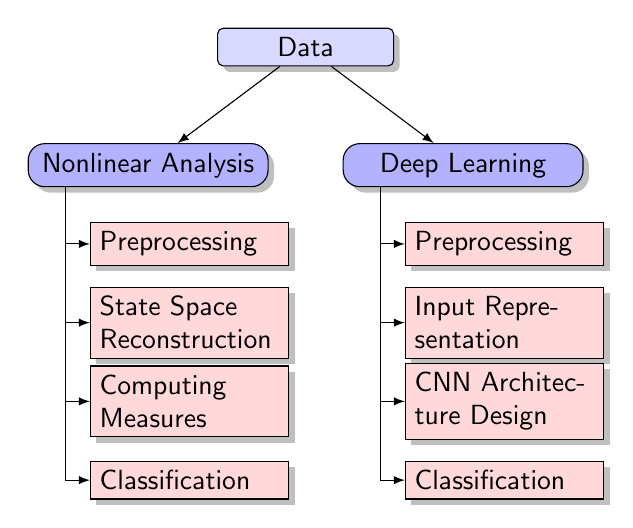
\begin{tikzpicture}[
  level 1/.style={sibling distance=40mm},
  edge from parent/.style={->,draw},
  >=latex]

% root of the the initial tree, level 1
\node[root] {Data}
% The first level, as children of the initial tree
  child {node[level 2] (c1) {Nonlinear Analysis}}
  child {node[level 2] (c2) {Deep Learning}};
  % child {node[level 2] (c3) {Drawing arrows between nodes}};

% The second level, relatively positioned nodes
\begin{scope}[every node/.style={level 3}]
\node [below of = c1, xshift=15pt] (c11) {Preprocessing};
\node [below of = c11] (c12) {State Space Reconstruction};
\node [below of = c12] (c13) {Computing Measures};
\node [below of = c13] (c14) {Classification};

\node [below of = c2, xshift=15pt] (c21) {Preprocessing};
\node [below of = c21] (c22) {Input Representation};
\node [below of = c22] (c23) {CNN Architecture Design};
\node [below of = c23] (c24) {Classification};
\end{scope}

% lines from each level 1 node to every one of its "children"
\foreach \value in {1,...,4}
  \draw[->] (c1.195) |- (c1\value.west);

\foreach \value in {1,...,4}
  \draw[->] (c2.195) |- (c2\value.west);

\end{tikzpicture}

\end{document}
